\documentclass[man, noextraspace]{apa6}
\usepackage{lmodern}
\usepackage{amssymb,amsmath}
\usepackage{ifxetex,ifluatex}
\usepackage{fixltx2e} % provides \textsubscript
\ifnum 0\ifxetex 1\fi\ifluatex 1\fi=0 % if pdftex
  \usepackage[T1]{fontenc}
  \usepackage[utf8]{inputenc}
\else % if luatex or xelatex
  \ifxetex
    \usepackage{mathspec}
  \else
    \usepackage{fontspec}
  \fi
  \defaultfontfeatures{Ligatures=TeX,Scale=MatchLowercase}
\fi
% use upquote if available, for straight quotes in verbatim environments
\IfFileExists{upquote.sty}{\usepackage{upquote}}{}
% use microtype if available
\IfFileExists{microtype.sty}{%
\usepackage{microtype}
\UseMicrotypeSet[protrusion]{basicmath} % disable protrusion for tt fonts
}{}
\usepackage{hyperref}
\hypersetup{unicode=true,
            pdftitle={Final Project: The Relationship between Sleep, Depression, Quality of Life, and Socioeconomic Status},
            pdfauthor={Alexis Adams-Clark, Andrew Fridman, \& Xi Yang},
            pdfkeywords={sleep, depression, quality of life, SES},
            pdfborder={0 0 0},
            breaklinks=true}
\urlstyle{same}  % don't use monospace font for urls
\usepackage{graphicx,grffile}
\makeatletter
\def\maxwidth{\ifdim\Gin@nat@width>\linewidth\linewidth\else\Gin@nat@width\fi}
\def\maxheight{\ifdim\Gin@nat@height>\textheight\textheight\else\Gin@nat@height\fi}
\makeatother
% Scale images if necessary, so that they will not overflow the page
% margins by default, and it is still possible to overwrite the defaults
% using explicit options in \includegraphics[width, height, ...]{}
\setkeys{Gin}{width=\maxwidth,height=\maxheight,keepaspectratio}
\IfFileExists{parskip.sty}{%
\usepackage{parskip}
}{% else
\setlength{\parindent}{0pt}
\setlength{\parskip}{6pt plus 2pt minus 1pt}
}
\setlength{\emergencystretch}{3em}  % prevent overfull lines
\providecommand{\tightlist}{%
  \setlength{\itemsep}{0pt}\setlength{\parskip}{0pt}}
\setcounter{secnumdepth}{0}
% Redefines (sub)paragraphs to behave more like sections
\ifx\paragraph\undefined\else
\let\oldparagraph\paragraph
\renewcommand{\paragraph}[1]{\oldparagraph{#1}\mbox{}}
\fi
\ifx\subparagraph\undefined\else
\let\oldsubparagraph\subparagraph
\renewcommand{\subparagraph}[1]{\oldsubparagraph{#1}\mbox{}}
\fi

%%% Use protect on footnotes to avoid problems with footnotes in titles
\let\rmarkdownfootnote\footnote%
\def\footnote{\protect\rmarkdownfootnote}


  \title{Final Project: The Relationship between Sleep, Depression, Quality of
Life, and Socioeconomic Status}
    \author{Alexis Adams-Clark\textsuperscript{1}, Andrew
Fridman\textsuperscript{1}, \& Xi Yang\textsuperscript{1}}
    \date{}
  
\shorttitle{Final Project}
\affiliation{
\vspace{0.5cm}
\textsuperscript{1} University of Oregon Department of Psychology}
\keywords{sleep, depression, quality of life, SES\newline\indent Word count: X}
\usepackage{csquotes}
\usepackage{upgreek}
\captionsetup{font=singlespacing,justification=justified}

\usepackage{longtable}
\usepackage{lscape}
\usepackage{multirow}
\usepackage{tabularx}
\usepackage[flushleft]{threeparttable}
\usepackage{threeparttablex}

\newenvironment{lltable}{\begin{landscape}\begin{center}\begin{ThreePartTable}}{\end{ThreePartTable}\end{center}\end{landscape}}

\makeatletter
\newcommand\LastLTentrywidth{1em}
\newlength\longtablewidth
\setlength{\longtablewidth}{1in}
\newcommand{\getlongtablewidth}{\begingroup \ifcsname LT@\roman{LT@tables}\endcsname \global\longtablewidth=0pt \renewcommand{\LT@entry}[2]{\global\advance\longtablewidth by ##2\relax\gdef\LastLTentrywidth{##2}}\@nameuse{LT@\roman{LT@tables}} \fi \endgroup}


\DeclareDelayedFloatFlavor{ThreePartTable}{table}
\DeclareDelayedFloatFlavor{lltable}{table}
\DeclareDelayedFloatFlavor*{longtable}{table}
\makeatletter
\renewcommand{\efloat@iwrite}[1]{\immediate\expandafter\protected@write\csname efloat@post#1\endcsname{}}
\makeatother
\raggedbottom
\setlength{\parskip}{0pt}

\authornote{ We would like to acknowledge Daniel Anderson for
introducing us to \texttt{papaja} and thank our classmates in
Introduction to Data Science with R.

Correspondence concerning this article should be addressed to Alexis
Adams-Clark, 1585 E 13th Ave, Straub 339, Eugene, OR 97403. E-mail:
\href{mailto:aadamscl@uoregon.edu}{\nolinkurl{aadamscl@uoregon.edu}}}

\abstract{
Depression is a widespread and debilitating mental illness. However,
sleep quality is a potent and modifiable protective factor that may
reduce depressive symptoms and increase quality of life. In this study,
we examined the associations among depressive symptoms, sleep quality,
and quality of life in a high risk sample. First, we assessed if there
are differences in depressive symptoms, sleep quality, and quality of
life according to socioeconomic status. Using correlational analyses, we
found depressive symptoms were negatively correlated with quality of
life and sleep quality. Meanwhile, sleep quality was positively
correlated with quality of life. The results indicate that intricate and
strong associations exist among depressive symptoms, sleep quality, and
quality of life. Clinical implications of these findings are also
discussed.


}

\usepackage{amsthm}
\newtheorem{theorem}{Theorem}[section]
\newtheorem{lemma}{Lemma}[section]
\theoremstyle{definition}
\newtheorem{definition}{Definition}[section]
\newtheorem{corollary}{Corollary}[section]
\newtheorem{proposition}{Proposition}[section]
\theoremstyle{definition}
\newtheorem{example}{Example}[section]
\theoremstyle{definition}
\newtheorem{exercise}{Exercise}[section]
\theoremstyle{remark}
\newtheorem*{remark}{Remark}
\newtheorem*{solution}{Solution}
\begin{document}
\maketitle

\section{Introduction}\label{introduction}

Sleep quality, typically indexed by a combination of sleep efficiency
and total sleep time (TST), is an important outcome in the context of
long-term health. Sleep efficiency is defined as the percentage of time
spent sleeping while laying in bed, whereas, total sleep time is the
amount of time spent sleeping, accounting for factors such as sleep
onset latency and awakenings. There is a multitude of studies that
suggesat that poor sleep is a prospective risk factor in premature
mortality (Knutson, Spiegel, Penev, \& Van Cauter, 2007). More
specifically, chronically disrupted and limited sleep has been linked to
increased rates of obesity, diabetes, cardiovascular disease, cognitive
impairment, and mental health disorders (Gangwisch, Malaspina,
Boden-Albala, \& Heymsfield, 2005).

Additionally, recent epidemiological research suggests that sleep has
continued to decrease over the past 30 years, which is consistent with
the significant increase in sleep-related complaints in the workforce
(Ferrie, Kumari, Salo, Singh-Manoux, \& Kivimäki, 2011). In this review
by Ferrie and colleagues, the reduction in sleep quality is also thought
to be associated with the staggering increase in work-related and
vehicular accidents. While research has provided evidence between sleep
quality and health-outcomes, there are few studies examining other
global measures such as quality of life.

Quality of life is a helpful and comprehensive measure of an
individual's subjective experience. For example, this variable may
encompass interpersonal and familial relationships, occupational
satisfaction, financial security, and intellectual development. While
there may be tangible health-related outcomes (e.g., number of hospital
visits), the subjective interpretation of distressing impairments due to
poor sleep quality may also provide valuable insights. This overall
outcome can adequately capture subthreshold depressive symptoms, which
may still benefit from various interventions (e.g., cognitive-behavioral
therapy for insomnia).

While this global measure may capture the negative impact of poor sleep
quality through broad strokes, depression is a more clinically-specific
outcome to consider. Depressive symptoms, such as low mood and
irritability, have been consistently linked to sleep-related
psychopathology (Spoormaker \& Bout, 2005). This pattern of poor sleep
quality may increase obstacles associated with obtaining reliable
treatment by exacerbating current depressive symptoms. Therefore, sleep
quality seems to be at the root of these domain-spanning impairments and
an essential target for intervention.

In this present study, we set out to evaluate evidence for the
association between sleep quality, depression, and quality of life in a
sample of diverse sample of adults. These relationships will also be
investigated in the context of low, medium, and high SES as a moderator,
as those in lower socioeconomic groups are at a higher risk for
depression and sleep problems. Given the importance of sleep quality and
mental health on long-term health outcomes, we hope to enrich the
current literature with a better understanding of these complex factors.
Findings from this study will inform models of psychopathology and
provide a foundation from which causal and longitudinal
intervention-focused research can be constructed.

\section{\texorpdfstring{Methods\footnote{This is a fictional Methods section, as we simulated our data. However, this is a realistic way that we could go about collecting this data in the future}}{Methods}}\label{methods}

\subsection{Participants}\label{participants}

Participants were recruited through Amazon Mechanical Turk (MTurk).
MTurk is a survey tool offered through Amazon.com, where people around
the world can complete surveys for monetary compensation. MTurk is
commonly used in social science research studies, and it has been found
to be representative.

In total, 500 participants were included in this study, all of whom had
complete data. Out of 500 participants, 194 identified as \enquote{low}
SES, 244 identified as \enquote{middle} SES, and 62 identified as
\enquote{high} SES. Out of 500 participants, 64 had not graduated high
school, 157 completed high school, 96 had a postsecondary certificate,
and 183 had some postsecondary education. Additionally, 344 identified
as European-American, 51 identified as African American, 51 identified
as Hispanic, 27 identified as Asian-American, 15 identified as American
Indian/Alaskan Native, 11 identified as Pacific Islander, and 1
identified as \enquote{other.}

\subsection{Materials}\label{materials}

\subsubsection{Depressive Symptoms
Scale}\label{depressive-symptoms-scale}

A scale to measure depressive symptoms was created by the researchers
for the purposes of this study. Participants were instructed to rate
each item on Likert-type scale, where 1 corresponds to \enquote{strongly
disagree,} and 5 corresponds to \enquote{strongly agree.} The scale
consisted of three items, including: \enquote{Over the last 2 weeks, I
have felt little interest or pleasure in doing things;} \enquote{Over
the last 2 weeks, I have felt down, depressed, or hopeless;} and
\enquote{Over the last 2 weeks, I have felt tired or had little energy.}
Scale items were summed to create a depression score, where higher
scores represent higher depressive symptoms.

\subsubsection{Quality of Life Scale}\label{quality-of-life-scale}

A scale to measure participants' quality of life was created by the
researchers. Participants were instructed to rate each item on
Likert-type scale, where 1 corresponds to \enquote{strongly disagree,}
and 5 corresponds to \enquote{strongly agree.} The scale consisted of
four items, including: \enquote{My life is ideal;} \enquote{I am
satisfied with my life;} \enquote{So far I have been able get the
important things I want from life;} and \enquote{I have accomplished
many of the things in my life.} Scale items were summed to create a
total quality of life score, where higher scores represent better
quality of life.

\subsubsection{Sleep Quality Scale}\label{sleep-quality-scale}

A scale to measure participants' sleep quality was created by the
researchers. Participants were instructed to rate each item on
Likert-type scale, where 1 corresponds to \enquote{strongly disagree,}
and 5 corresponds to \enquote{strongly agree.} The scale consisted of
three items, including: \enquote{I am satisfied with the time I spend
sleeping;} \enquote{I am satisfied with my quality of sleep}; and
\enquote{When I wake up, I feel refreshed.} Scale items were summed to
create a total sleep quality score, where higher scores represent better
sleep quality.

\subsubsection{Demographics
Questionnaire}\label{demographics-questionnaire}

Participants were also asked to complete a demongraphics questionnaire,
which asked about their socioeconomic status, race/ethnicity, and
educational background.

\subsection{Procedure}\label{procedure}

An online version of this study was created through Qualtrics survey
software, and the survey link was distributed to participants on the via
Amazon Mechanical Turk. The study was advertised as \enquote{a study of
sleep and well-being.} After clicking the survey link, participants were
informed of study procedures and content through an informed consent
process. After completing the study, participants received academic
credit as compensation and were presented with debriefing materials. The
University of Oregon's s Office of Research Compliance (Institutional
Review Board) approved this study.

\subsection{Data analysis}\label{data-analysis}

We used R (Version 3.4.3; R Core Team, 2017) and the R-packages
\emph{\}cowplot} {[}@\}R-cowplot{]}, \emph{bindrcpp} (Version 0.2.2;
Müller, 2018), \emph{dplyr} (Version 0.7.6; Wickham, François, Henry, \&
Müller, 2018), \emph{forcats} (Version 0.3.0; Wickham, 2018a),
\emph{Formula} (Version 1.2.3; Zeileis \& Croissant, 2010),
\emph{ggplot2} (Version 3.0.0; Wickham, 2016), \emph{gridExtra} (Version
2.3; Auguie, 2017), \emph{here} (Version 0.1; Müller, 2017),
\emph{Hmisc} (Version 4.1.1; Harrell Jr, Charles Dupont, \& others.,
2018), \emph{janitor} (Version 1.1.1; Firke, 2018), \emph{kableExtra}
(Version 0.9.0; Zhu, 2018), \emph{knitr} (Version 1.20; Xie, 2015),
\emph{lattice} (Version 0.20.35; Sarkar, 2008), \emph{papaja} (Version
0.1.0.9842; Aust \& Barth, 2018), \emph{purrr} (Version 0.2.5; Henry \&
Wickham, 2018), \emph{readr} (Version 1.1.1; Wickham, Hester, \&
Francois, 2017), \emph{rio} (Version 0.5.10; C.-h. Chan, Chan, Leeper,
\& Becker, 2018), \emph{stringr} (Version 1.3.1; Wickham, 2018b),
\emph{survival} (Version 2.42.6; Terry M. Therneau \& Patricia M.
Grambsch, 2000), \emph{tibble} (Version 1.4.2; Müller \& Wickham, 2018),
\emph{tidyr} (Version 0.8.1; Wickham \& Henry, 2018), and
\emph{tidyverse} (Version 1.2.1; Wickham, 2017) for all our analyses. We
calculated means and standard deviations for each of the total scale
scores, and we separated means by socioeconomic status. We also
calculated Pearson's r correlation coefficients between depressive
symptoms, quality of life, and sleep quality total scores. The authors
interpreted our correlational results as small (.10-.29), medium
(.30-.49), and large correlations (.50-1.00).

\section{Results}\label{results}

\begin{table}[tbp]
\begin{center}
\begin{threeparttable}
\caption{\label{tab:Table 1}Mean Depression, Sleep Quality, and Quality of Life Scores by SES Group.}
\begin{tabular}{cccc}
\toprule
SES & \multicolumn{1}{c}{Mean Depression Score} & \multicolumn{1}{c}{Mean Sleep Quality Score} & \multicolumn{1}{c}{Mean Quality of Life Score}\\
\midrule
High & 7.37 & 9.94 & 7.74\\
Low & 7.34 & 10.03 & 7.66\\
Med & 7.72 & 9.86 & 7.45\\
\bottomrule
\addlinespace
\end{tabular}
\begin{tablenotes}[para]
\normalsize{\textit{Note.} This table was created with apa\_table()}
\end{tablenotes}
\end{threeparttable}
\end{center}
\end{table}

\begin{figure}
\centering
\includegraphics{APA_Document_files/figure-latex/plot 1-1.pdf}
\caption{}
\end{figure}

\subsection{Descriptive Statistics}\label{descriptive-statistics}

The mean depression total score for the sample is 7.53 . The mean sleep
quality total score for the sample is 9.94. The mean quality of life
total score for the sample is 7.57. Mean total scores separated by
socioeconomic status are listed in Table 1 and graphically displayed in
Figure 1.

\subsection{Correlation Results}\label{correlation-results}

Depressive symptoms, sleep quality, and quality of life scores were
significantly correlated with each other, \emph{p} \textless{} .05 (see
Table 2).

\subsection{Exploratory Analyses in Low SES
Individuals}\label{exploratory-analyses-in-low-ses-individuals}

In order to look at these relationships specifically in Low SES
individuals, we plotted the correlations between depressive symptoms,
sleep quality, and quality of life in only low SES individuals (see
Figure 2). To look sepcifically at the differences in scores on each
depressive symptom, we subtracted the scores of low SES individuals from
high SES individuals and plotted the differences (see Figure 3)

\begin{table}[tbp]
\begin{center}
\begin{threeparttable}
\caption{\label{tab:table2}Correlations between Depression, Sleep Quality, and Quality of Life Scores.}
\begin{tabular}{llll}
\toprule
row & \multicolumn{1}{c}{column} & \multicolumn{1}{c}{cor} & \multicolumn{1}{c}{p}\\
\midrule
Sleep Quality & Depression & -0.20 & 0.00\\
Sleep Quality & Quality of Life & 0.22 & 0.00\\
Depression & Quality of Life & -0.55 & 0.00\\
\bottomrule
\addlinespace
\end{tabular}
\begin{tablenotes}[para]
\normalsize{\textit{Note.} This table was created with apa\_table()}
\end{tablenotes}
\end{threeparttable}
\end{center}
\end{table}

\begin{figure}
\centering
\includegraphics{APA_Document_files/figure-latex/plot 2-1.pdf}
\caption{}
\end{figure}

\begin{figure}
\centering
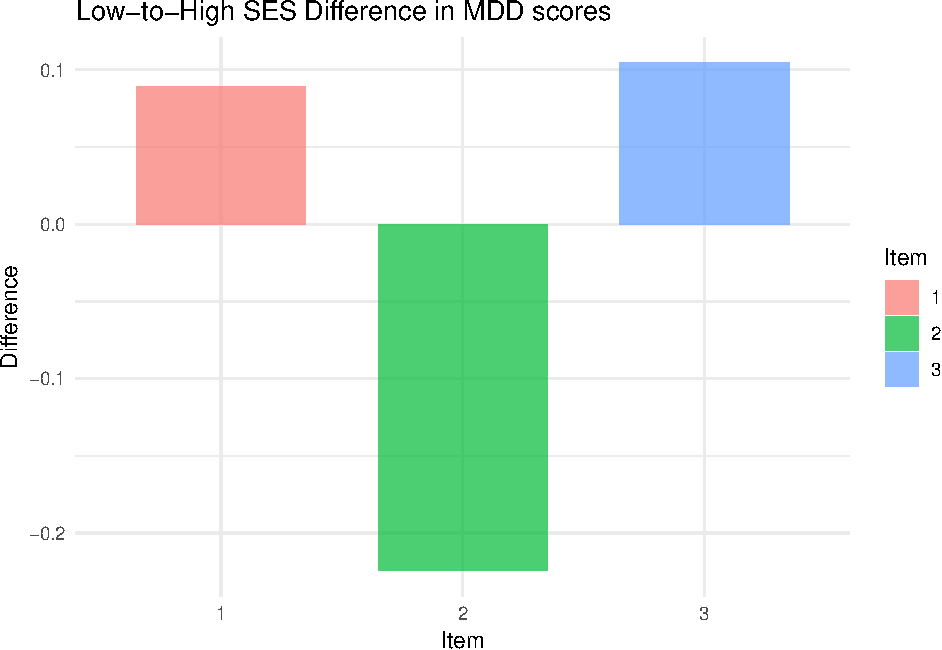
\includegraphics{APA_Document_files/figure-latex/Figure 3-1.pdf}
\caption{}
\end{figure}

\section{Discussion}\label{discussion}

Our results confirmed that more depression symptoms were correlated with
lower life quality and sleep quality. Whereas sleep quality was
positively associated with life quality. The results were consistent
with past literature and our hypothesis. Based on the symptoms from
major depressive disorder diagnosis, a patient suffering from depression
is likely to experience either hypersomnia or insomnia. Insomnia is most
related to low sleep quality. Meanwhile, hypersomnia does not guarantee
high sleep quality as much too long duration of sleep may cause
dizziness and lethargy in the patients. In reverse, frequent sleep
disturbances and the discomfort and stress that come with low sleep
quality may negatively impact a patient's everyday mood and reduce the
general energy level to engage in more mood-boosting activities. These
bidirectional influences may explain the negative correlation between
depression and sleep quality that we detected with our sample. As sleep
is an instrumental component in everyday life, lower sleep quality will
inevitably decrease life quality. Higher life quality may consist of
more comfortable sleeping environment and less sleep-hindering stress.
These potential connections help elucidate the positive association
between sleep quality and life quality. Limitations of our study lie in
our correlational study design such that we were unable to examine
causal relationship among the variables. We also relied on self-report
measures which may be susceptible to reporter bias. Possible bias in
this high risk sample include underreport depression symptoms due to low
insight or emotional numbness, as well as overreporting symptoms due to
Hawthorne effect or other motivations. In studies to follow, we will
also adopt structured clinical interview and objective measures of the
key variables. We will incorporate sleep intervention (e.g., insomnia
cognitive behavior therapy) to manipulate the sleep quality level to
examine causal relationship between depression symptoms and sleep
quality. An active and a waitlist control groups will be recruited to
rule out more confounds. More sophisticated statistical analyses such as
multilevel modeling may be adopted. Clinical implications from the
results may inform clinicians and the general public to pay more
attention to sleep quality with an aim of keeping depression at bay or
reducing depressive symptoms. In general, our study with a high risk
sample demonstrated the intricate associations among depressive
symptoms, sleep and life quality.

\newpage

\section{References}\label{references}

\begingroup
\setlength{\parindent}{-0.5in} \setlength{\leftskip}{0.5in}

\hypertarget{refs}{}
\hypertarget{ref-R-gridExtra}{}
Auguie, B. (2017). \emph{GridExtra: Miscellaneous functions for ``grid''
graphics}. Retrieved from
\url{https://CRAN.R-project.org/package=gridExtra}

\hypertarget{ref-R-papaja}{}
Aust, F., \& Barth, M. (2018). \emph{papaja: Create APA manuscripts with
R Markdown}. Retrieved from \url{https://github.com/crsh/papaja}

\hypertarget{ref-R-rio}{}
Chan, C.-h., Chan, G. C., Leeper, T. J., \& Becker, J. (2018).
\emph{Rio: A swiss-army knife for data file i/o}.

\hypertarget{ref-ferrie2011sleep}{}
Ferrie, J. E., Kumari, M., Salo, P., Singh-Manoux, A., \& Kivimäki, M.
(2011). Sleep epidemiology---a rapidly growing field. Oxford University
Press.

\hypertarget{ref-R-janitor}{}
Firke, S. (2018). \emph{Janitor: Simple tools for examining and cleaning
dirty data}. Retrieved from
\url{https://CRAN.R-project.org/package=janitor}

\hypertarget{ref-gangwisch2005inadequate}{}
Gangwisch, J. E., Malaspina, D., Boden-Albala, B., \& Heymsfield, S. B.
(2005). Inadequate sleep as a risk factor for obesity: Analyses of the
nhanes i. \emph{Sleep}, \emph{28}(10), 1289--1296.

\hypertarget{ref-R-Hmisc}{}
Harrell Jr, F. E., Charles Dupont, \& others. (2018). \emph{Hmisc:
Harrell miscellaneous}. Retrieved from
\url{https://CRAN.R-project.org/package=Hmisc}

\hypertarget{ref-R-purrr}{}
Henry, L., \& Wickham, H. (2018). \emph{Purrr: Functional programming
tools}. Retrieved from \url{https://CRAN.R-project.org/package=purrr}

\hypertarget{ref-knutson2007metabolic}{}
Knutson, K. L., Spiegel, K., Penev, P., \& Van Cauter, E. (2007). The
metabolic consequences of sleep deprivation. \emph{Sleep Medicine
Reviews}, \emph{11}(3), 163--178.

\hypertarget{ref-R-here}{}
Müller, K. (2017). \emph{Here: A simpler way to find your files}.
Retrieved from \url{https://CRAN.R-project.org/package=here}

\hypertarget{ref-R-bindrcpp}{}
Müller, K. (2018). \emph{Bindrcpp: An 'rcpp' interface to active
bindings}. Retrieved from
\url{https://CRAN.R-project.org/package=bindrcpp}

\hypertarget{ref-R-tibble}{}
Müller, K., \& Wickham, H. (2018). \emph{Tibble: Simple data frames}.
Retrieved from \url{https://CRAN.R-project.org/package=tibble}

\hypertarget{ref-R-base}{}
R Core Team. (2017). \emph{R: A language and environment for statistical
computing}. Vienna, Austria: R Foundation for Statistical Computing.
Retrieved from \url{https://www.R-project.org/}

\hypertarget{ref-R-lattice}{}
Sarkar, D. (2008). \emph{Lattice: Multivariate data visualization with
r}. New York: Springer. Retrieved from
\url{http://lmdvr.r-forge.r-project.org}

\hypertarget{ref-spoormaker2005depression}{}
Spoormaker, V. I., \& Bout, J. van den. (2005). Depression and anxiety
complaints; relations with sleep disturbances. \emph{European
Psychiatry}, \emph{20}(3), 243--245.

\hypertarget{ref-R-survival-book}{}
Terry M. Therneau, \& Patricia M. Grambsch. (2000). \emph{Modeling
survival data: Extending the Cox model}. New York: Springer.

\hypertarget{ref-R-ggplot2}{}
Wickham, H. (2016). \emph{Ggplot2: Elegant graphics for data analysis}.
Springer-Verlag New York. Retrieved from \url{http://ggplot2.org}

\hypertarget{ref-R-tidyverse}{}
Wickham, H. (2017). \emph{Tidyverse: Easily install and load the
'tidyverse'}. Retrieved from
\url{https://CRAN.R-project.org/package=tidyverse}

\hypertarget{ref-R-forcats}{}
Wickham, H. (2018a). \emph{Forcats: Tools for working with categorical
variables (factors)}. Retrieved from
\url{https://CRAN.R-project.org/package=forcats}

\hypertarget{ref-R-stringr}{}
Wickham, H. (2018b). \emph{Stringr: Simple, consistent wrappers for
common string operations}. Retrieved from
\url{https://CRAN.R-project.org/package=stringr}

\hypertarget{ref-R-tidyr}{}
Wickham, H., \& Henry, L. (2018). \emph{Tidyr: Easily tidy data with
'spread()' and 'gather()' functions}. Retrieved from
\url{https://CRAN.R-project.org/package=tidyr}

\hypertarget{ref-R-dplyr}{}
Wickham, H., François, R., Henry, L., \& Müller, K. (2018). \emph{Dplyr:
A grammar of data manipulation}. Retrieved from
\url{https://CRAN.R-project.org/package=dplyr}

\hypertarget{ref-R-readr}{}
Wickham, H., Hester, J., \& Francois, R. (2017). \emph{Readr: Read
rectangular text data}. Retrieved from
\url{https://CRAN.R-project.org/package=readr}

\hypertarget{ref-R-knitr}{}
Xie, Y. (2015). \emph{Dynamic documents with R and knitr} (2nd ed.).
Boca Raton, Florida: Chapman; Hall/CRC. Retrieved from
\url{https://yihui.name/knitr/}

\hypertarget{ref-R-Formula}{}
Zeileis, A., \& Croissant, Y. (2010). Extended model formulas in R:
Multiple parts and multiple responses. \emph{Journal of Statistical
Software}, \emph{34}(1), 1--13.
doi:\href{https://doi.org/10.18637/jss.v034.i01}{10.18637/jss.v034.i01}

\hypertarget{ref-R-kableExtra}{}
Zhu, H. (2018). \emph{KableExtra: Construct complex table with 'kable'
and pipe syntax}. Retrieved from
\url{https://CRAN.R-project.org/package=kableExtra}

\endgroup


\end{document}
